\section{The Nugget Framework}\label{sec:the_nugget_framework}

Nugget is designed to address the limitations of the prior sampling techniques, specifically focusing on 1) the high cost of finding samples, 2) the coupling of the samples to a specific executable binary, and 3) the infeasibility of validating the selected samples.
Nugget leverages LLVM passes to statically insert annotations to analyze the program's execution on real hardware without the need for simulation, emulation, or binary translation.
By using LLVM intermediate representation (IR) to define program progress and intervals, the samples become independent of the binary and can be reused across different executable versions of the same program, since LLVM IR abstracts away details of the final binary.
Lastly, Nugget provides a method to create portable samples to be executed on any platform, such as real hardware or simulators, so that the samples can be validated in native time with real hardware before running them on a simulator.

\begin{figure}[!t]
    \centering
    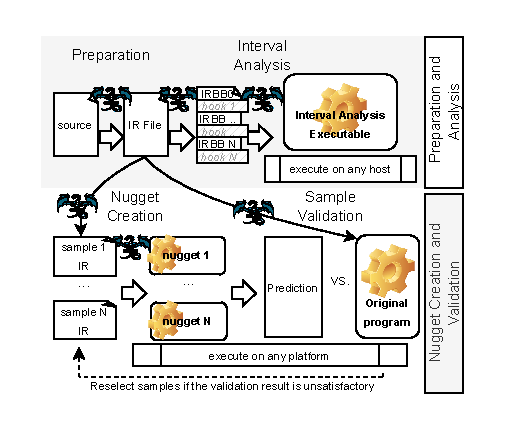
\includegraphics[width=\columnwidth]{images/index_delayed_ui.pdf}
    \caption{Nugget pipeline. The process is divided into two main stages:
    (1) preparation and analysis, and
    (2) nugget selection and validation.
    The preparation and analysis stage, including base IR file creation and interval analysis execution, needs to be performed only once per program.
    Nugget creation and validation can be repeated to refine and select the most representative set of samples for the workload.}
    \label{fig:nugget_pipeline}
\end{figure}
\FloatBarrier

In this section, we present an overview of Nugget as a pipeline (Figure~\ref{fig:nugget_pipeline}), describing its workflow from preparation through interval analysis, nugget creation, and finally, sample selection verification.
It is not the focus of this thesis to introduce a new sample selection algorithm, but rather to provide a framework that can be used to implement and validate diverse sample selection methodologies that can be tailored to specific applications and workloads.

\revision{We begin by defining program progress and intervals, which ensures that samples remain independent of the binary, as described in Section~\ref{sec:unit_of_work}.}
Next, we describe the preparation required by Nugget to guarantee the LLVM IR of the program remains consistent across different binaries in Section~\ref{sec:initial_setup}.
Then, we introduce our novel interval analysis methodology, which leverages LLVM passes, enabling comprehensive program analysis directly on real hardware without imposing hardware-specific constraints in Section~\ref{sec:interval_analysis}.
Following that, we present the nugget creation process, which allows for the generation of portable samples that can be executed on any platform, including real hardware and simulators, in Section~\ref{sec:nugget_creation}.
Finally, we describe the sample selection validation process, which enables efficient validation of the selected samples for specific workloads in native time, ensuring that the samples accurately represent the program's execution in Section~\ref{sec:verification}.

